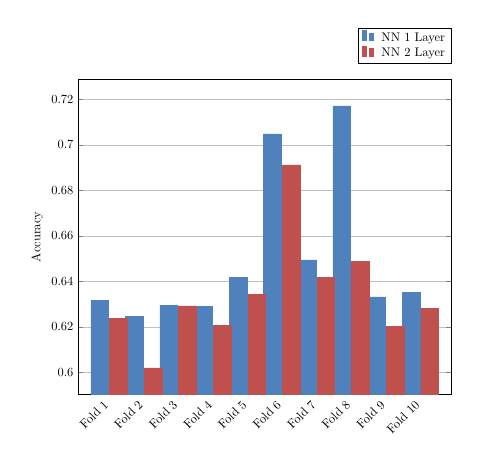
\begin{tikzpicture}[scale=0.45]

\definecolor{bblue}{HTML}{4F81BD}
\definecolor{rred}{HTML}{C0504D}

    \begin{axis}[
        width  = 1.0*\textwidth,
        major x tick style = transparent,
        ybar=2*\pgflinewidth,
        bar width=0.5cm,
        ymajorgrids = true,
        ylabel = {Accuracy},
        symbolic x coords={Fold 1, Fold 2, Fold 3, Fold 4, Fold 5, Fold 6, Fold 7, Fold 8, Fold 9, Fold 10},
        xtick = data,
        legend cell align=left,
        legend style={
                at={(1,1.05)},
                anchor=south east,
                column sep=1ex
        },
        x tick label style={font=\normalsize, rotate=45, anchor=east}
    ]
        \addplot[style={bblue,fill=bblue,mark=none}]
            coordinates {(Fold 1, 0.63154) (Fold 2, 0.62454) (Fold 3,0.62951) (Fold 4, 0.62887) (Fold 5, 0.64158) (Fold 6, 0.70474) (Fold 7, 0.64938) (Fold 8, 0.71709) (Fold 9, 0.63316) (Fold 10, 0.63501)};

        \addplot[style={rred,fill=rred,mark=none}]
             coordinates {(Fold 1, 0.62362) (Fold 2, 0.60188) (Fold 3, 0.62915) (Fold 4, 0.62049) (Fold 5, 0.6344) (Fold 6, 0.69111) (Fold 7, 0.64182) (Fold 8, 0.64864) (Fold 9, 0.62008) (Fold 10, 0.6281)};

        \legend{NN 1 Layer, NN 2 Layer}
    \end{axis}
\end{tikzpicture}